\section{Non-equilibrium Work: A Corrective Framework}
\label{app:nonequilibrium}

This development branch supplies a mathematically specified correction, not a
reinterpretation of the archived molecular results or a claim of a new work
identity. Jarzynski's relation and its single-molecule pulling applications
\citep{jarzynski1997master,hummerszabo2001}, escorted transport
\citep{escorted2008}, stochastic normalizing flows \citep{snf2020}, and FEAT
\citep{feat2025} are direct prior work. Microsoft's enhanced diffusion sampling
\citep{enhanceddiffusion2026} uses steering and unbiasing relative to a pretrained
model distribution; taking that distribution as the equilibrium reference does
not establish that our FM model matches an independently specified eSEN target.

\paragraph{Generalized work and the BGFM residual.}
Fix composition, charge and spin, an orthonormal coordinate system on $H$, and
a potential $U$ including any declared confinement, with
$0<Z=\int_H e^{-\beta U(x)}\,dx<\infty$. Translation removal alone does not
ensure this condition. For a normalized prior $q_0$ and an invertible map
$x_1=\Phi_\theta(x_0)$, change of variables gives the dimensionless work
\begin{equation}
w=\beta U(x_1)+\log q_0(x_0)-\log|\det D\Phi_\theta(x_0)|
 =\beta U(x_1)+\log q_\theta(x_1).
\end{equation}
Consequently $\E_{q_0}[e^{-w}]=Z$ and
$\E_{q_\theta}[w]+\log Z=\KL(q_\theta\Vert\pi)$, where
$\pi=e^{-\beta U}/Z$. This identifies the \emph{ideal} residual as generalized
work. The archived readout is not a validated $\log q_\theta$, and variance
within disconnected off-policy clouds is neither this ensemble average nor a
constraint on global basin masses. The time parameter of an artificial
transport need not be physical molecular-dynamics time.

\paragraph{A finite-step path identity.}
Let the implemented forward path have density
$Q(x_{0:K})=q_0(x_0)\prod_{k=1}^K K_k(x_k\mid x_{k-1})$.
Choose normalized auxiliary backward kernels $L_k(x_{k-1}\mid x_k)$ and assume
the resulting target path measure is absolutely continuous with respect to $Q$.
The weight
\begin{equation}
 a(x_{0:K})=
 \frac{e^{-\beta U(x_K)}}{q_0(x_0)}
 \prod_{k=1}^K\frac{L_k(x_{k-1}\mid x_k)}
                         {K_k(x_k\mid x_{k-1})}
 \label{eq:finitework}
\end{equation}
satisfies $\E_Q[a f(x_K)]=\int_H e^{-\beta U(x)}f(x)\,dx$ for integrable $f$.
Indeed, multiplying by $Q$ cancels every forward factor; integrating the
normalized backward kernels successively leaves the stated endpoint integral.
This is ordinary path importance sampling, as used in
\citet{snf2020,feat2025}, rather than a new theorem.

Gaussian forward and backward kernels give evaluable finite-step factors
without a CNF trace. Their means may use learned flow velocities; neither
kernel needs to be the exact physical dynamics. They must describe the
actual sampled state, including the coordinate measure. The implementation
therefore uses explicit Euclidean coordinates and an orthonormal basis for
the molecular COM-free subspace. It also implements the value-only AIS
reference \citep{neal2001ais}, with work updates before Metropolis moves
invariant to each annealed density.

\paragraph{Noise and sampling efficiency are separate issues.}
An unbiased log estimate is not an unbiased exponential weight:
if $\widehat{\log q}=\log q+\epsilon$ and
$\epsilon\mid x\sim\mathcal N(0,s(x)^2)$, then
$\E[e^{-\epsilon}\mid x]=e^{s(x)^2/2}$.
For two states with true masses $(0.2,0.8)$ and variances $(0,2)$, naive noisy
reweighting gives limiting second-state mass
$0.8e/(0.2+0.8e)\simeq0.9158$. Independent replica products correct a quadratic
objective; they do not remove this exponential bias. We therefore do not use
the stochastic CNF readout as an exact work weight.

Exact weight formulas also do not imply useful effective sample size.
We report $(\sum_i a_i)^2/\sum_i a_i^2$ and the maximum normalized weight.
The raw mean weight estimates $Z$ without bias under the assumptions; its
logarithm and self-normalized observables have finite-sample bias. Weighted
endpoint clouds may supervise conditional flow matching by pairing endpoints
with independent Gaussian starts and interpolation times. The distilled
student is approximate and requires its own evaluation.

\paragraph{Evidence scope.}
New tests enumerate every path of a finite-state non-reversible example,
recover constant work for an exactly reversible Gaussian step, and check AIS
Gaussian moments and normalization, energy-offset invariance, intrinsic
coordinate measure and weighted-CFM gradients. A five-seed, known-target
mixture experiment compares unweighted paths, terminal-energy-only weighting,
AIS correction and matched FM distillation. This is an implementation and
mechanism experiment; it supplies no molecular improvement or novelty claim.
Promotion to the main empirical contribution requires matched molecular
oracle budgets, adequate ESS, independent evaluation and verified source
metadata, all beyond the mathematical identity.

\paragraph{Completed development results.}
With $8{,}192$ particles and $16$ AIS stages in each of five seeds, the target
right-basin mass is $0.8$. Mean occupancies are $0.5089$ for unweighted paths,
$0.8039$ for terminal-energy-only weighting and $0.7982$ for AIS weights.
Mean squared distance to the nearest mode is respectively $1.9616$, $0.3011$
and $0.4854$, against target $0.5$: energy-only weighting happens to get the
occupancy close while overconcentrating the within-basin distribution.
Mean AIS ESS is $10.99\%$ of the particle count.
Matched 1,000-update FM students trained on unweighted/weighted teachers attain
occupancies $0.4996/0.7630$ and spreads $1.8380/0.7113$.
Thus the weighted teacher helps this toy student, but distillation does not
preserve exact target statistics.
\begin{figure}[ht]
\centering
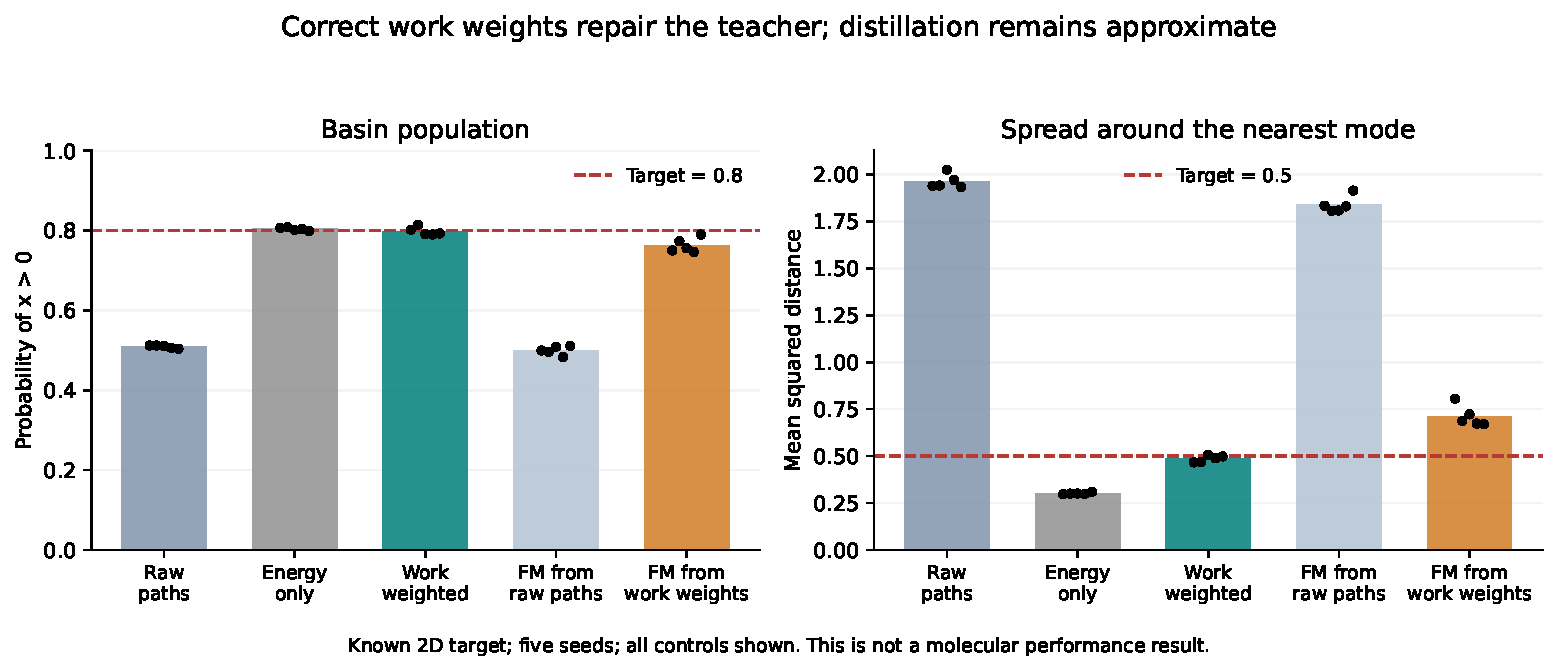
\includegraphics[width=\linewidth]{figures/nonequilibrium_toy.pdf}
\caption{Known-target development control. Bars are means and points show all
five seeds. Red lines are the target statistics. Neither this established
AIS mechanism nor the toy improvement establishes a new molecular method.}
\label{fig:nonequilibriumtoy}
\end{figure}

A first real-model pilot freezes the smoothed displacement FM checkpoint and
uses 32 Gaussian paths with 32 steps, noise scale $0.1$, and auxiliary backward
drift $-v$. The fixed eight-atom validation condition (processed row 5846) has
recorded charge $+1$ and declared singlet multiplicity; original spin metadata
is unavailable. All 32 eSEN evaluations are finite. The declared target is
restrained, $U=E_{\rm eSEN}+0.05\sum_i\|x_i\|^2$ in eV, with $kT=1$ eV.
The resulting ESS is only $1.655/32$ and one endpoint carries $72.87\%$ of the
weight. This establishes executable two-environment inference, while exposing
poor weight efficiency. It is insufficient for a molecular sampling or
generation-advantage claim and does not justify promoting this branch to the
main empirical result.

\paragraph{Raw-source recovery and corrected electronic states.}
Subsequent recovery of the public 4M archive provides 3,986,754 original records.
Replaying preprocessing matches all 3,941,522 accepted records bitwise in the
legacy coordinates, atom types, charge features, forces and rounded energies.
Original charge, spin and float64 energies are retained in separate sidecars.
There are 72,423 charges outside the old feature range and 678,514 non-singlets;
403,895 records have multiplicity above the minimum allowed by electron parity.
An explicit global-state adapter therefore supplies total charge and multiplicity
to the geometry model, replacing the atom-zero total-charge marker.
Matched 10,000-update data-FM continuations, with and without that adapter,
both give 32/32 successful xTB evaluations at the original electronic states.
Median strain is 3.9438 versus 3.8931 eV, respectively.
This is an electronic-state correction, not demonstrated quality improvement.

\paragraph{Independent thermodynamic reference.}
For the neutral AgBr2 doublet (validation row 1137, verified raw row 118392),
rotation-reduced randomized-Sobol integration using analytic Gaussian proposals
gives $\log\widehat Z=144093.1276$ at 3,072 points per scramble and four
independent scrambles. The estimated relative standard error is $1.67\%$,
larger than the final resolution change of 0.00146 nat. It is a statistical
reference rather than exact truth. In three-seed direct importance sampling
with 1,024 potential queries per seed, the confinement Gaussian attains mean
weight ESS 233.85 and mean absolute log-normalizer error 0.05897 nat.
The defensive ordinary and symmetry-averaged template mixtures attain ESS
44.52 and 90.35, with errors 0.15055 and 0.09840 nat. Thus symmetry averaging
helps the template proposal in this experiment but does not surpass the simple
Gaussian reference proposal. The harder eight-atom system remains strongly
weight-degenerate. Neither corrected theory nor these implementation checks
establish improved molecular generation or converged sampling on the broader
system panel.
